%% LyX 2.2.1 created this file.  For more info, see http://www.lyx.org/.
%% Do not edit unless you really know what you are doing.
\documentclass[twoside,english]{elsarticle}
\usepackage[T1]{fontenc}
\usepackage[latin9]{inputenc}
\pagestyle{headings}
\usepackage{babel}
\usepackage{prettyref}
\usepackage{amsmath}
\usepackage{graphicx}
\usepackage[unicode=true,
 bookmarks=true,bookmarksnumbered=false,bookmarksopen=false,
 breaklinks=false,pdfborder={0 0 0},pdfborderstyle={},backref=false,colorlinks=false]
 {hyperref}

\makeatletter
\@ifundefined{date}{}{\date{}}
%%%%%%%%%%%%%%%%%%%%%%%%%%%%%% User specified LaTeX commands.
\usepackage{url}
% specify here the journal
\journal{ Electric Power Systems Research}

% use this if you need line numbers
%\usepackage{lineno}

\makeatother

\begin{document}

\begin{frontmatter}{}

\title{Distance Protection Zone 3 Misoperation During System Wide Cascading
Events: The Problem and a Survey of Solutions}

\author[rvt]{A.M.~Abdullah\corref{cor1}}

\ead{ahmad.abdullah@cu.edu.eg}

\author[focal]{K.~Butler-Purry}

\ead{klbutler@tamu.edu}

\cortext[cor1]{Corresponding author}

\address[rvt]{Department of Electrical Power and Machines, Cairo University, Gizah,
Egypt, 12613}

\address[focal]{Department of Electrical and Computer Engineering, Texas A\&M University,
College Station, TX, 77843}
\begin{abstract}
Distance relay zone 3 misoperation has been responsible for major
blackouts around the world. Zone 3 misoperation generally occurs under
system wide cascading events such as the 2003 Northeastern US-Canada
blackout or under stressed system conditions such as the 2015 Turkish
blackout. This paper explains the problem of zone 3 distance protection
misoperation. The paper then proceeds to survey the literature for
possible solutions to increase distance relay security to prevent
distance protection misoperation. Three categories of solutions were
proposed in literature to address the problem of zone 3 distance protection
misoperation. The first one is anticipation and prevention of misoperation
in the planning stage. The second one is communication assisted protection
schemes that use remote measurements to enhance relay security. The
last one uses local data to enhance distance relay security. 
\end{abstract}
\begin{keyword}
Distance protection zone 3 \sep blackouts \sep cascading events
\sep misoperation \sep security 
\end{keyword}

\end{frontmatter}{}

\section{Introduction\label{sec:Introduction}}

With the deregulated market structure in the United States and Europe,
grid operators are under more pressure to reap more profits of existing
infrastructure due to increased competition. The grid is thus increasingly
operated near the threshold of stability. Failure of the grid, better
known as blackouts, carries catastrophic economic and societal sequences.
Large blackouts tend to be due to either extreme natural events such
as hurricanes or a series of events called cascading failures \citep{Hines2009}.
In this paper, we only focus on cascading events. Those events can
be any of the following: line tripping, overloading of other lines,
malfunctions of protection systems, power oscillations and voltage
instability \citep{Yamashita}. The reason that is considered in this
paper is distance protection misoperation which is a contributing
factor in seventy percent of all cascading events \citep{Chen2005}.
If not discovered and mitigated in an early stage, cascading events
generally lead to a complete blackout. With today\textquoteright s
society much dependence on electricity as a form of energy, preventing
such damage is of high importance. 

Cascading failures are defined as \textquotedblleft a sequence of
dependent failures of individual components that successively weaken
the power system\textquotedblright{} \citep{Baldick}. Since the 2003
US-Canada blackout, cascading events have drawn much attention in
the industrial and academic community. Even though the world has witnessed
many blackouts prior to the 2003 blackout \citep{Hines2009}, the
dramatic causes and consequences of the 2003 blackout have left industrial
and academic community with the burden of exploring this phenomenon
in more detail. To understand the severity of the 2003 blackout \citep{Liscouski2004},
it sufficient to say it had caused the loss of 62 GW which caused
the lights to turn off for more than 51 million people in the eastern
interconnection. Considering the many components and the bits and
pieces involved, a domino effect of events evolved slowly (hours)
or fast (seconds) according to the region causing a degradation of
the integrity of the system leading ultimately to a complete blackout.
The main reason of the 2003 blackout was distance relay misoperation.
Daunting efforts had to be exerted to gain more knowledge and understanding
of the underlying phenomenon. 

Relays by design act quickly to remove the fault from the system by
disconnecting faulted lines. However, sometimes relays fail to perform
such function which is considered a protection system misoperation.
Of all protection system misoperations that lead to cascading events,
this paper focuses exclusively on distance protection misoperation.
A protection system misoperation is defined as ``a failure to operate
as intended for protection purposes'' \citep{NERCMisoperation}.
Various categories are given for misoperation in \citep{NERCMisoperation}.
However, in this paper the word misoperation will be used exclusively
to mean only one of them, namely, an operation in which a protection
system trips a healthy line due to heavy loading when no fault exists.
In other words, other causes of distance protection misoperation such
as power swing are not considered in this paper. Notable cascading
events \citep{Yamashita,Novosel2004} begin with lines that were tripped
due to actual faults. The tripping of those faulty line causes the
current flowing in those lines to be redistributed to adjacent lines.
Those lines may be overloaded and thus tripped incorrectly -protection
misoperation- which may trigger a sequence of cascading events that
might ultimately lead to a blackout. It should be noted that regardless
of the initial triggering events- whether a fault or not- that cause
cascading events, historically those cascading events were triggered
under stressful system conditions \citep{Liscouski2004,Kosterev1999}.

As mentioned in \citep{Yamashita}, one of the effective ways to prevent
cascading events is to specify potential undesirable relay operations
ahead of time. In this paper, we show that even though distance protection
misoperation can be anticipated ahead of time, prevention of this
misoperation is not possible with distance protection principle only
because the distance protection principle is not able to be selective
in some regions of its operation. 

The paper is organized as follows: Section \eqref{sec:Typical-Distance-Protection}
provides a sample distance relay that is set according to NERC standards.
Once this relay is set according to NERC directives, it will be explained
in the same section that the relay may still misoperate under various
operating conditions. Anticipation and detection of distance relay
misoperation in the planning stage is described \prettyref{sec:Detection-and-mitigation-of-cascading-events-in-the-planning-stage}.
\prettyref{sec:Communication-Assisted-Schemes} provides an overview
of the communication assisted schemes that have been proposed to eliminate
the distance protection misoperation. Lastly, \prettyref{sec:Modifications-to-Local}
offers a survey on the methods that were suggested in literature to
enhance the distance protection security using local data only. 

\section{The Distance Protection Misoperation Problem\label{sec:Typical-Distance-Protection}}

On August 14th of 2003 \citep{Liscouski2004}, the US eastern interconnection
suffered one of the largest blackouts in the recent US history. Three
345 kV transmission lines sagged into untrimmed trees during the hot
summer days. The tripping of those lines caused another 345 kV transmission
line to carry substantial system load. The heavy loading of this last
line coupled with relatively low system voltage, caused the distance
relay to confuse a heavy loading situation for uncleared zone 3 fault
as the impedance entered the third zone of protection which in turn
resulted in tripping of the heavily loaded line. The tripping of the
healthy yet heavily loaded line worsened system conditions leading
to a chain of events that ultimately led to system collapse. Also,
on March 31st of 2015 \citep{2015Turkish}, the Turkish grid suffered
the worst blackout ever recorded since 1999 when an earthquake caused
a complete shutdown of the grid. On the contrary to the 1999 earthquake,
the 2015 blackout was caused by a impedance protection misoperation
that tripped a heavily loaded line on the 400 kV transmission level
even though there was no fault on the tripped line or anywhere in
the transmission network. As can be seen from the examples in \citep{Liscouski2004,2015Turkish}
in which distance protection misoperation have been the main cause
of the blackouts or in \citep{Abdullah} in which distance protection
misoperation have been studied in the IEEE 118 bus system , a distance
protection misoperation is characterized by a distance protection
system seeing a heavy load on a line as a fault. This confusion arises
from the fact that the impedance measured by the impedance protection
system coincides with that of a fault. The reason for the heavy load
can be due to load shifting after a fault as in the 2003 US-Canada
blackout \citep{Liscouski2004} or due to lines out of service for
maintenance causing one line to carry substantial system power transfer
as in the 2015 Turkish blackout \citep{2015Turkish} or due to any
unforeseen reasons. 

To illustrate that this confusion is not tied up with certain system
conditions but rather inherent insecurity in the distance protection
principle, the single line diagram shown in Figure \ref{fig:System-Configuration-for-formulating-problem}
is used to formulate the problem in general terms. It will be shown
below that this insecurity always exists and the degraded system conditions
only excite it; that is, for some regions in the impedance protection
zone the protection system is not able to be selective between a fault
and non-fault condition. Without the degraded system conditions, it
is highly unlikely that a distance protection misoperates. Even though,
degraded system conditions can be anticipated in the planning stage,
the system operator will have nothing in hand to prevent a distance
protection misoperation if local function of the distance protection
is used alone. It is important to keep in mind that distance protection
systems are set locally with the help of the impedance of adjacent
lines without any information about the system load until the coordination
study phase. In the coordination study phase, the transmission line
owner checks all settings against applicable standards. This is explained
in detail in \citep{thompson2015transmission}. In the following paragraphs,
we will set up the relay settings first then discuss what happens
in system wide cascading events.

In Figure \ref{fig:System-Configuration-for-formulating-problem},
the distance protection relay that will be studied is the relay at
point A of line A-C. Line A-C is connected to three (3) lines, namely
C-M, C-N and C-P. The number of lines connected to line A-C will not
affect zone 1 or zone 2 settings but will affect zone 3 settings.
As will be seen below, tripping in Zone 3 becomes more insecure with
more lines connected to line A-C as zone 3 reach becomes larger. To
simplify the analysis, all lines are assumed to have the same impedance
as well as the short circuit level. However, as will be explained
below, this simplification does not affect the generality of the problem
formulation. The impedance and the rating of the lines are $60$ $\varOmega$
and 3000 Amp, respectively and are taken from \citep{NERC2003}. The
setting of zone 1 is assumed to be 0.85 of the line impedance. Zone
2 setting is assumed to be 1.2 of the line impedance. However, some
consideration is needed to set the third zone. The third zone has
to be set such that it can protect the longest adjacent line (assumed
to be line C-P in this case) and to protect 20\% beyond that line
to provide backup to the remote circuit breakers. In case of a bolted
three phase fault on line C-P and assuming that the short circuit
contributions of all buses is given in Figure \ref{fig:System-Configuration-for-formulating-problem}
by $I_{index}$ where $index$ is the bus name (being M , N, A or
P), the voltage at distance protection system at A can be written
as given in equation \prettyref{eq:VoltageAtRelat}.
\begin{figure}[h]
\begin{centering}
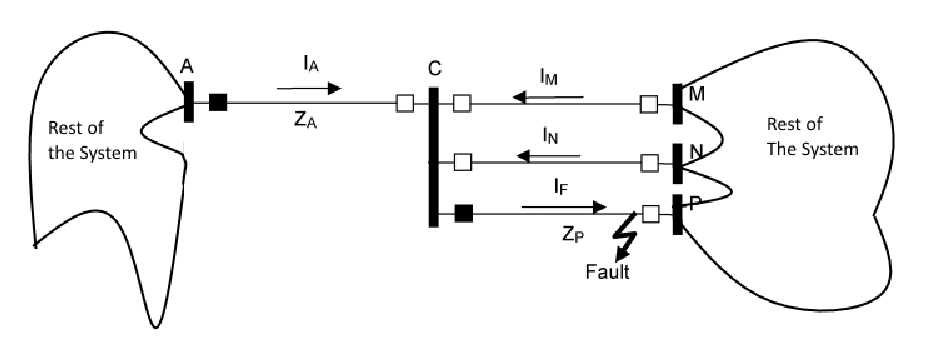
\includegraphics[scale=0.6]{fig1}
\par\end{centering}
\caption[System Configuration for formulating the problem]{System Configuration for formulating the problem\label{fig:System-Configuration-for-formulating-problem}}
\end{figure}

\begin{equation}
V_{A}=I_{A}\times Z_{A}+Z_{P}\times\left(I_{M}+I_{A}+I_{N}\right)\label{eq:VoltageAtRelat}
\end{equation}

The impedance that is seen by the relay A can then be written as in
\prettyref{eq:ApparentImpedanceAtRelay}

\begin{equation}
Z_{R}=\frac{V_{A}}{I_{A}}=Z_{A}+Z_{P}\left(1+\frac{I_{M}+I_{N}}{I_{A}}\right)\label{eq:ApparentImpedanceAtRelay}
\end{equation}

Equation \prettyref{eq:ApparentImpedanceAtRelay} will only be applicable
to faults on line C-P, if we need to include 20\% for the line that
is beyond bus P, then the impedance $Z_{P}$ in \prettyref{eq:ApparentImpedanceAtRelay}
has be replaced by $1.2\times Z_{P}$. Using the data in \citep{NERC2003}
and assuming all lines are identical as well as their short circuit
contribution, then the setting of zone 3 will be $Z_{A}+3.6\times Z_{P}=4.6\times Z_{A}$.
The three zones are plotted in Figure \ref{fig:Distance-Relay-characteristic}.
\begin{figure}[!h]
\centering{}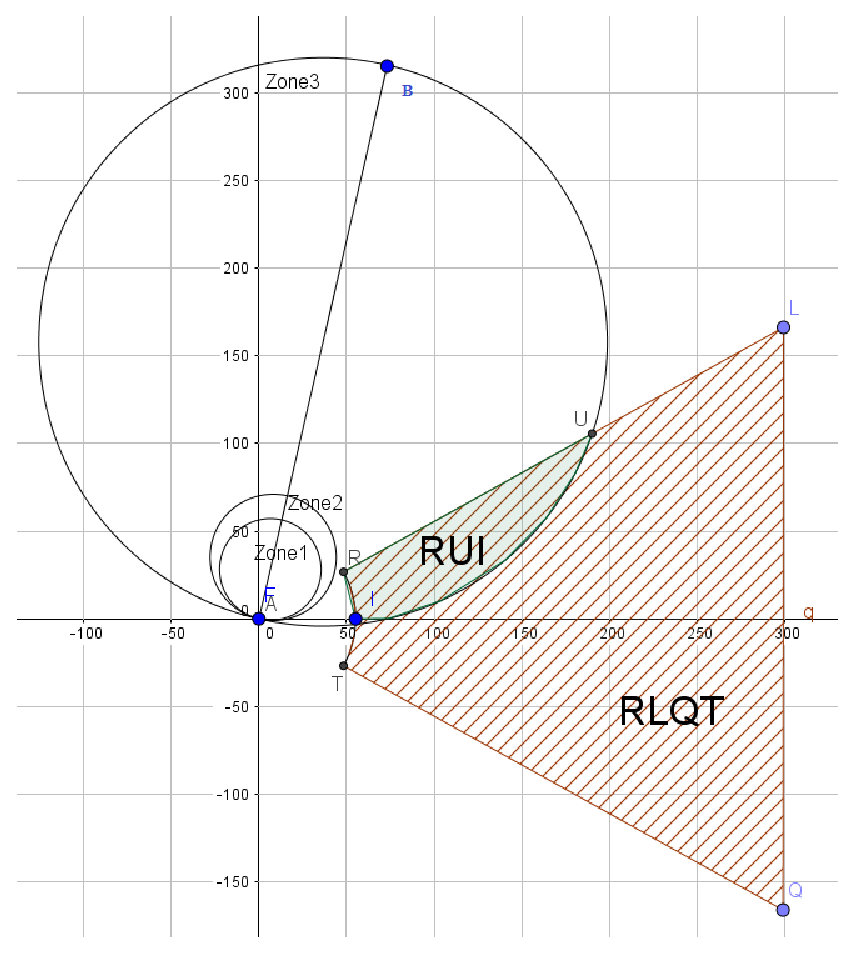
\includegraphics[scale=0.6]{fig2}\caption[Distance protection characteristic ]{Distance protection characteristic for system in Figure \ref{fig:System-Configuration-for-formulating-problem}
\textbf{\label{fig:Distance-Relay-characteristic}}}
\end{figure}
 

After setting up the relay locally, applicable standards and directives
need to be applied to the settings for compliance purposes. This step
involves running worst case power flow in the summer peak case. The
most notable directive is the load encroachment. The load encroachment
zone is an area of the protection zone in which the load impedance
\textquotedblleft{} encroaches\textquotedblright{} \textendash intrudes-
upon the fault impedance. Load encroachment will obviously cause misoperation
and should be removed from the zone of protection \citep{NERC2003}.
To plot the load encroachment zone according to NERC directives \citep{NERCMisoperation,NERC2003,NERCLoadability},
the load zone should include the point which corresponds to 150\%
line loading and 0.85 per unit voltage. Thus the load encroachment
locus of the distance relay at A will consist of two parts. The first
part will be an arc of circle of radius given in equation \prettyref{eq:LoadImpedance}
which is given as arc \textbf{RIT} in Figure \ref{fig:System-Configuration-for-formulating-problem}.
This arc \textbf{RIT} corresponds to the least impedance that the
relay should not issue a trip command for. The other characteristic
load lines will be two lines making an angle of $\pm30^{\circ}$ with
the x-axis ($\pm30^{\circ}$ represents the power factor of the line
under worst case loading condition)

\begin{equation}
Z_{load}=\frac{V_{A}}{I_{A}}=\frac{\frac{345kV}{\sqrt{3}}\times0.85}{1.5\times3000}=57\varOmega\label{eq:LoadImpedance}
\end{equation}

The orange hashed area \textbf{RLQT} is the load encroachment area.
NERC directives \citep{NERCMisoperation,NERC2003,NERCLoadability}
states that this load encroachment zone has to be removed from the
relay operating zone. It can be seen at once that if the impedance
seen by the relay lies within the solid green area \textbf{URI} then
a relay may confuse this operating point for a fault since the point
lies already in zone 3. This confusion arises if the fault resistance
is high enough to cause the fault point to lie within the solid green
area \textbf{URI}. In Figure \ref{fig:Distance-Relay-characteristic},
this fault resistance ranges from $30$$\varOmega$ to $90$$\varOmega$.
The fault resistance can be obtained by measuring the distance between
the diameter \textbf{AB} of zone 3 circle to point \textbf{R} and
\textbf{U} of the green zone. If it is known in advance that the fault
resistance calculated cannot be attained along the route of the transmission
line, then the risk of misoperation is nonexistence and the green
area can be removed from zone 3 without affecting the security or
reliability of the distance protection system. However, fault resistance
along the route of the transmission line is not known in advance.
Also, one should note that solid state and electromechanical relays
can not be programmed, only microprocessor relays can. This really
means that older relays will have to comply with NERC standards by
disabling zone 3 altogether. It is shown in \citep{Horowitz2006}
that disabling zone 3 in some cases will force protection engineers
to provide back up protection solutions to remote circuit breakers.
This might involve a considerable cost. Additionally, not all countries
around the world have standards as strict as NERC, so the solid green
area \textbf{URI }exist in the zone of protection without regard from
the protection engineer. Lastly, even if the relay complies with NERC
directives, an impedance can still fall anywhere in zone 3, not only
the solid green area \textbf{URI,} under stressed system conditions
as Phadke and Horowitz pointed out in their paper \citep{Horowitz2006}.
This shows clearly the impedance protection is inherently insecure
under stressed system conditions. 

Attention is now given to the assumptions stated in the beginning.
It was assumed that all lines have the same impedance and all of them
are contributing equal currents to the fault. It can be seen at once
from Figure \ref{fig:Distance-Relay-characteristic} that this assumption
is not restricting the generality of the problem formulation. Because
in any case the green area \textbf{URI} will exist due to the load
profile under stressed conditions. Additionally, the fault contribution
of the transmission lines will only affect the diameter \textbf{BA}
of zone 3 which will only affect point \textbf{U}. Point \textbf{U}
correspond to the max fault resistance. Stated differently, there
will always be an overlap between the dynamic rating of the line and
zone 3 and the short circuit levels from nearby lines will only affect
the size of the overlap (area \textbf{URI)} not the overlap itself.
Lastly, to derive equations \prettyref{eq:VoltageAtRelat} and \prettyref{eq:ApparentImpedanceAtRelay},
a three phase fault has been assumed. This is due to the fact that
line overload is three phase phenomenon. However, it should not be
hard to be able to envision a single line to ground fault causing
the same effect if one important line is operated with only one phase
due to a line to line fault under heavy loading conditions. 

It should be apparent from the description above that the major issue
that is faced by traditional impedance protection system is that the
steady state impedance corresponding to a heavy load is coincident
to the impedance under a fault on a remote line to which the distance
protection system provides backup protection. It could be argued that
impedance protection should be supervised by other steady state protection
principles to enhance its selectivity, i.e, the ability to differentiate
between a load and a fault current. However, other protection principles
-such as over current protection- that can make the distinction between
a load and a fault depend on the anticipated power flow for operation
while the problem in hand is different. The confusion that is seen
by the distance protection is because the power flow under system
wide cascading failures changes considerably from the planned power
flow. In other words, the load encroachment zone has to be set for
system wide cascading scenarios that are not known in advance, which
is close to impossible undertaking. One of the authors \citep{Horowitz2006}
states this fact as:

\textit{\textquotedbl{}The overwhelming thrust of the NERC rules and
other instructions regarding the application of zone 3 elements has
been to prevent its operation during emergency conditions. Although
this is a desirable goal, it should be recognized that even with all
the intelligence available to modern computer relays, the problem
of distinguishing a fault from a heavy load in a relatively short
time and using only the current and voltage signals available to the
relay can not be solved in every single imaginable (and some unimaginable)
power system scenarios\textquotedbl{}}.

\section{Detection and mitigation of zone 3 misoperation in the planning stage\label{sec:Detection-and-mitigation-of-cascading-events-in-the-planning-stage}}

Most Independent System Operators (ISOs) \citep{ERCOTNodal,CaisoPlanning}
today use N-1 criterion to judge whether the system is secure after
the removal of one line in planning stage. However, given that zone
3 distance protection misoperation is not triggered until two or three
lines go out of service \citep{Liscouski2004}, the distribution of
power flow is hard to be taken into account in the planning stage
as it would mean performing N-2 and N-3 contingency analysis which
is expensive computationally. Thus, it is increasingly hard to assess
protection system capability under the most stressful system conditions.\textsl{
}Due to that, the authors in \citep{li2007operation,li2008sensitivity}
provided an efficient method to study the sensitivity of zone 3 under
various operating conditions without the need for performing large
number of power flow studies. In \citep{li2007operation,li2008sensitivity},
the authors define a linearized impedance margin of a distance relay
using system voltages, injected power and shunt susceptance. The impedance
margin is defined as the distance between the measured impedance locus
in the R-X plane to the boundary of the operating characteristic of
the relay and is shown in Figure \ref{fig:Impedance-margin-and}.
By doing so, the relays that may misoperate can be anticipated ahead
of time in an efficient manner in the planning stage using simple
formulas. However, it is shown in the paper that if the changes in
the voltages or power injections are electrically far away from the
relay under study, a situation that always exists in wide area cascading
scenarios, the error in the analysis becomes unacceptable especially
for long lines. 
\begin{figure}[h]
\begin{centering}
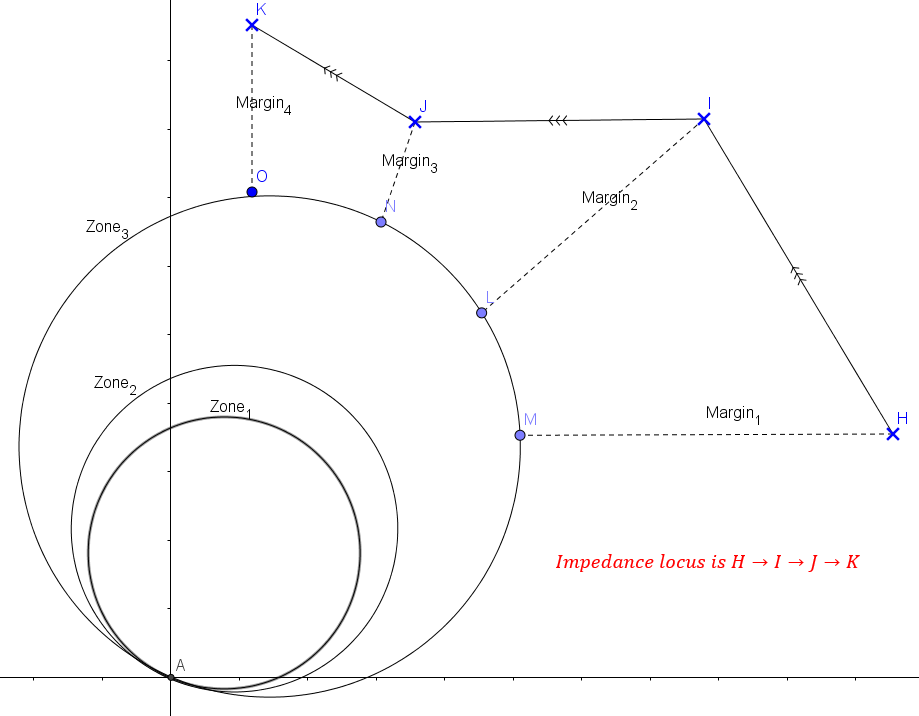
\includegraphics[scale=0.6]{fig3}\caption{Impedance margin and impedance locus plot for a distance relay during
a wide area cascading scenario\label{fig:Impedance-margin-and}}
\par\end{centering}
\end{figure}

In \citep{aghamohammadi2016new}, the authors propose blocking zone
3 of certain distance relays ahead of time based on offline simulations.
The authors propose that the system operator perform contingency analysis
using credible historical contingencies in planning stage to observe
the impedance trajectory at each distance relay in the system. The
contingency scenarios to be performed have to include more than one
contingency to create an impedance trajectory. The relays that misoperate
during each contingency scenario due to the impedance trajectory entering
zone 3 when no fault conditions exist should be short listed. Of those
relays that are short listed, certain relays are selected such that
their zone 3 protection will be disabled. The relays that will be
disabled are common to all contingency scenarios and are selected
based on a specific criterion explained in the paper. However, the
contingency scenarios can be hard to design in the planning stage
for modern power systems that have thousands of buses. Additionally,
disabling zone 3 effectively disables backup protection for remote
circuit breaker which is a situation that should be avoided unless
another form of backup is available. 

The authors in \citep{Song2007} proposed certain indices that can
accurately gauge the severity of system conditions and the likelihood
of cascades in real time. An index that is used to monitor distance
relays is also proposed. If the indies associated with the distance
relays exceed their threshold, then distance protection misoperation
is about to occur and the system operator has the option to stop distance
relays from operation. However, in practice only N-1 contingencies
are studied and thus the severity index is chosen based on these cases.
Nevertheless, if the system enters N-2 or N-3 contingency conditions,
tuning of the \textquotedblleft severity\textquotedblright{} threshold
will be a difficult task computationally. 

Lastly, distance protection co-ordination has been explored in \citep{ravikumar2008approach,ravikumar2009approach}.
An SVM for each relay is trained using the impedance trajectory that
is seen by the relay during fault conditions. The impedance trajectory
is obtained by using a transient stability program. SVM is then trained
for various scenarios to distinguish zone 1, zone 2 and zone 3 faults.
Training scenarios include cases for different fault types at different
distances away from the relay that has the SVM and at different fault
resistances. Testing scenarios for SVM include faults that have not
used in training. By ensuring that the relays are well co-coordinated
under various contingency conditions, unnecessary trip could be avoided.
However, the impedance trajectory will depend on the system topology
at the time of fault occurrence and this has not been taken into consideration
in \citep{ravikumar2008approach,ravikumar2009approach} which could
lead to large offline training set. 

Due to the fact that distance protection co-ordination requires large
amount of offline simulations by performing many contingency conditions,
the authors in \citep{tasdighi2016automated} introduced the idea
of ``distance of impact'' to automate the distance protection co-ordination.
However, the authors use the super computer to perform their computations
at the first stage. Once the distance of impact of each relay has
been calculated, co-ordination of the distance relays becomes straight
forward. A shortcoming of the distance co-ordination approach is that
even though it can ensure that distance relays never overreach for
faults beyond their reach, little research has been performed to study
whether the co-ordination can ensure that relays will not misoperate
under heavy loading conditions. 

\textbf{As can be seen above, anticipation detection  of distance
protection misoperation in the planning stage is a hard task. To be
able to fully prevent distance protection misoperation, an N-x, where
x is greater than 1, contingency analysis need to be done. Even though
this could be done for small benchmark systems, contingency analysis,
under uncertain load and generation, is computationally intensive
for large system consisting of thousands of buses. Many ISOs may not
have access to supercomputers to run such intensive computations. }

\section{Communication Assisted Schemes\label{sec:Communication-Assisted-Schemes}}

The 2003 blackouts pointed out the importance of having events along
with the time they occurred. Investigators spent much of their time
trying to match up the waveforms to reconstruct the sequence of events
that led to the blackout. It was then apparent that to facilitate
the transfer and comparison of waveforms, all samples need to have
a time stamp for this purpose. Phasor Measurement Unit (PMU) or synchrophasor
technology was then recommended to address this shortcoming \citep{Liscouski2004}.
By the time of 2003 blackout, state estimation was a very mature field,
but PMUs opened new areas for the application of state estimation
by reducing the time needed to do state estimation due to wide spread
deployment in the transmission network. A PMU measures the positive
sequence voltage and current (both the magnitude and angle), which
opens new areas for adaptive relaying and wide area control and protection.
In typical distance protection schemes, the relay is only applied
to a single transmission line. However, in a wide area protection
scheme, a complete area (several transmission lines) can be protected
using selected PMU devices without the need to apply PMUs to each
single bus in the system. By transferring information in between PMUs
in the power system, accurate decision regarding the nature of the
impedance falling in zone 3 can be made and misoperation can be avoided.

With the introduction of PMUs, several fault detection and locations
methods have been proposed. The salient feature of PMU detection schemes
\citep{Joe-Air2000} is that using the communication links to transfer
data between the two ends of the lines, several conclusions can be
drawn regarding whether the line is undergoing abnormal conditions.
A salient feature of the PMU algorithm is the ability to monitor the
status of the line and compute the parameters of the line online in
a very accurate way. 

Due to the fact that zone 3 of distance relays may not be able differentiate
between heavy line load and an actual fault on the system, the authors
in \citep{Lim2008} proposed that a tool be installed at the control
center, also known as Independent System Operator (ISO), to continuously
supervise the operation of zone 3 elements. The tool will consist
of two modules, a central control unit (CCU) and several regional
control units (RCUs) as shown in Figure \ref{fig:RCU-and-CCU}. The
CCU will be installed in the ISO while the RCUs will be installed
at select individual substations. The CCU measures the line outage
distribution factors and generation shift factors for the entire power
grid and sends all factors to the individual RCUs. RCUs use local
measurements at the substation and communicate with one another. The
individual RCUs will differentiate between faults and transfer of
power flow and supervise distance relays based on the information
received from the CCU and other RCUs. Even though this solution might
be able to prevent all zone-3 misoperations, it needs considerable
cost to construct the communication infrastructure that is needed
to transmit the data between the individual substation and the ISO.
\begin{figure}[h]
\begin{centering}
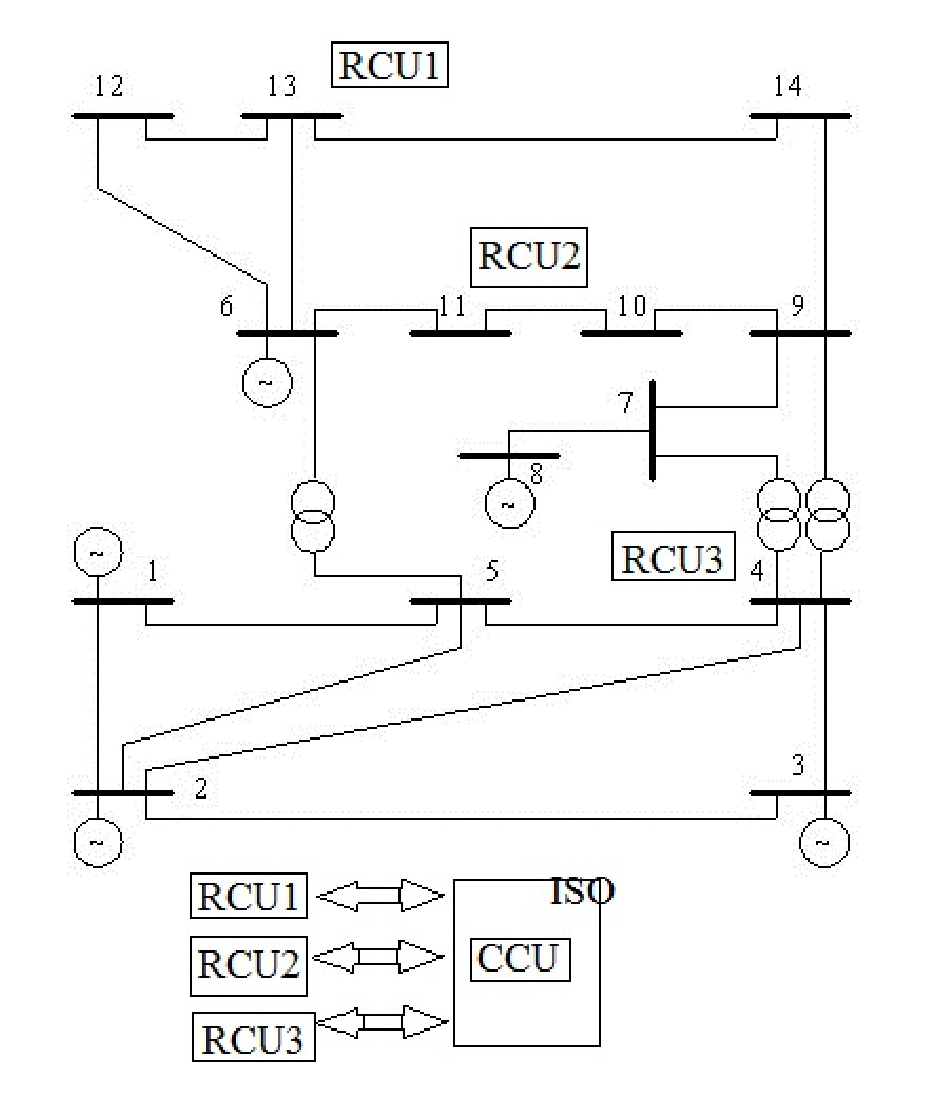
\includegraphics[scale=0.7]{fig4}\caption{RCU and CCU of the solution in \citep{Lim2008}\label{fig:RCU-and-CCU} }
\par\end{centering}
\end{figure}

The authors in \citep{dutta2014transmission} uses synchronized samples
from both ends of the line to check whether the transmission line
has been tripped successfully or not. The instantaneous power from
both line ends are calculated. It is shown in the paper that after
fault inception, the instantaneous power at both ends becomes positive.
This hold true even under systems with week infeed. The method is
applicable to all systems other than radial systems. However, due
to the need to transfer data between both ends, significant cost may
be incurred to establish such algorithm across each transmission line
in the grid. The approach that has been proposed in \citep{dutta2014transmission}
has been validated using field data in \citep{esmaeilian2015transmission}. 

In \citep{navalkar2011secure}, distributed PMUs are used to reach
a definitive decision about the existence of the fault in the system
using a synchrophasor state estimator (SynSE). The SynSE is used to
detect network topology changes as well as determine the fault locations
as shown in Figure \ref{fig:Protection-logic-ofSYNSE}. However, the
grid has be completely observable by PMUs. Thus, siting PMUs has to
be done carefully to not create unobservable islands under stressed
system conditions and certain contingency conditions. 
\begin{figure}[h]
\begin{centering}
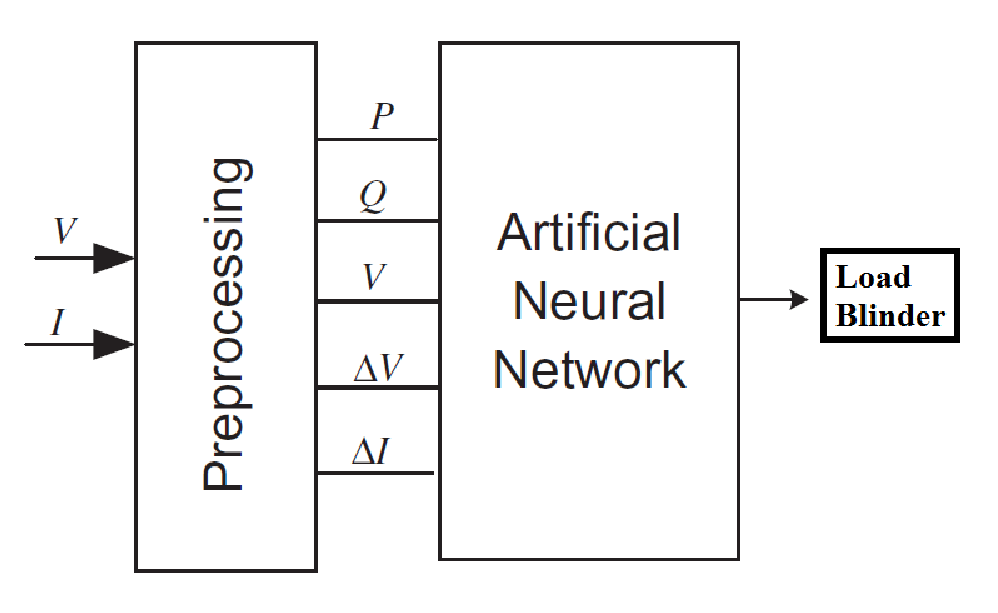
\includegraphics[scale=0.5]{fig5}\caption{Protection logic of the paper in \citep{navalkar2011secure}\label{fig:Protection-logic-ofSYNSE} }
\par\end{centering}
\end{figure}

In \citep{Kundu2014} synchrophasors are proposed to supervise zone
3 operation. Specific indices are proposed to assert the fault using
the currents which result in a very robust zone 3 distance protection
system. The algorithm forms a super node from the certain groups of
PMUs. By summing the current going into the super node, a decision
can be reached whether a disturbance exists or not. If a disturbance
is detected, another logic is invoked to determine whether it is a
fault for the group of PMUs with the higher deviation. The logic that
is invoked after disturbance detection is impedance based. A weighted
fault detection index is defined for this purpose. The weights used
to define the index depend on the reach of the respective zone 3 distance
protection relay. If after disturbance detection, the weighted fault
index is exceeded, a fault in zone 3 is declared and the relay is
restrained from operation. However, to fully take advantage of the
method, strategically located PMUs have to exist in the system which
makes the approach highly dependent on the topology and any transmission
system upgrades. Additionally, certain contingency conditions can
cause some faults not to be detected due to the location of the PMUs. 

In \citep{Garlapati2013}, agents are used to aid zone 3 relay elements
without enforcing a decision. In this scheme, each impedance relay
will have the capability to communicate with other agents in the network
that protect the same transmission line. If the majority of the agents
informs the local distance relay that the impedance in its zone 3
reach is actually due to a fault, then the local distance relay should
be energized and a trip command has to be issued. An optimization
approach is set up such that the communication delay between the various
agents are less than 1 second, which is the time of operation of zone
3. A similar approach has been proposed in \citep{haj2014intelligent}
where agents are installed everywhere without the optimization approach. 

In \citep{Neyestanaki2015}, a limited number of PMUs are used to
determine the faulted line as well as the location of the fault. An
optimization approach is used to locate a set of PMUs such that the
observability is independent of the generator models. A backup protection
zone is then constructed using the lines and buses between each PMU
such that a line in not included in two regions. The sum of zero and
positive sequence currents are used as discriminant for fault detection
and location. If the sum is not zero then the area will be flagged
as having a fault. Next comes the task of identifying the faulted
line. For the area that is flagged as having a fault, a distance quantity
will be calculated for each line within the area, i.e., each line
will be assumed faulted and a distance quantity will be calculated.
If the distance quantity falls between 0 to 1 then the faulted line
will be determined. If more than one line is found to be faulted,
an estimation of relative residual error is made and the line with
the minimum residual error will be selected as the faulted line. It
is clear from this description that two faults within any protected
zone or cross country faults will be detected as one fault only. And
even though one of the two faults may have not been cleared, the algorithm
may not be able to detect such situation. 

In \citep{Eissa2010}, a backup wide area protection scheme is proposed.
Short window DFT is used to extract the phasor information from the
three phase voltages and currents. In this scheme, the absolute difference
of the bus angles and currents are used to detect the fault. The minimum
voltage magnitude establishes the closest bus to the fault and the
maximum current angle difference between the buses establishes the
faulted lines. However, for the method to work, the minimum voltage
threshold has to be established. It is shown in the paper that a voltage
threshold less than 0.95 means that there is a fault on a system.
This immediately points out that in case of voltage instability conditions,
the method can operate erroneously.

In \citep{He2011}, another wide area protection scheme is proposed.
The solution consists of two components: a fault element identification
(FEI) and a fault area detection (FAD). The FEI is used to identify
the faulted element in the zone being protected. After that, the fault
isolation is realized by coordination among area circuit breakers
breakers. As part of the FEI, the measured voltage and current of
one terminal of the protected area are used to estimate the voltages
at the other end. If an internal fault occurs within the zone being
monitored, then the estimated value will be different from the measured
value at that bus causing a fault to be detected. On the other hand,
the faulted area is detected through FAD. The substations that are
within the faulted area need to send the information to the central
control room. Afterwords, the central control room will search the
suspected faulty lines and identify actual faulty lines quickly. The
use of FAD concept reduces the communication overhead required by
the scheme. The overall structure of the solution is shown in Figure
\ref{fig:The-concept-of-FAD}. 
\begin{figure}[h]
\begin{centering}
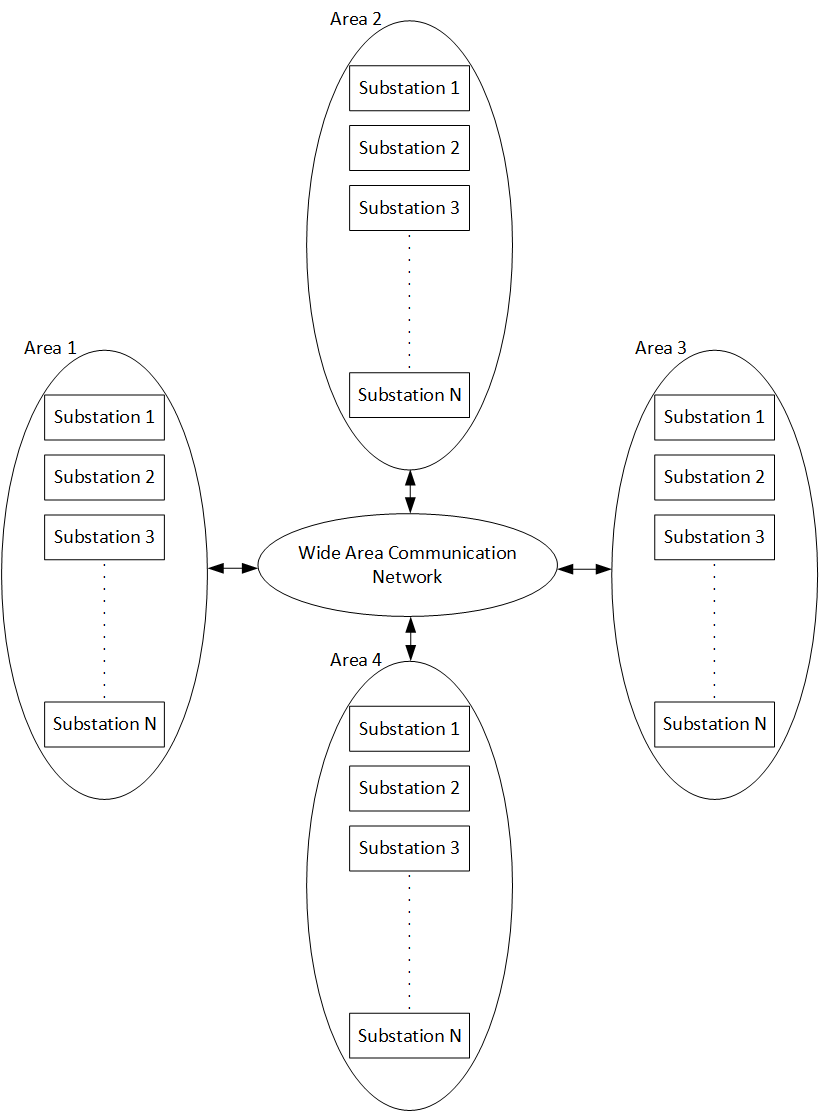
\includegraphics[scale=0.5]{fig6}
\par\end{centering}
\caption{The concept that is given in \citep{He2011}. A select number of substations
will be included in the communication network. \label{fig:The-concept-of-FAD}}
\end{figure}

The authors in \citep{lin2016countermeasures} use PMUs, that are
in place as part of a wide area protection scheme, to detect the power
flow transfer due to the removal of faulted line from service. In
\citep{lin2016countermeasures}, the load flow transfer to a line
can be calculated using the network topology via the distribution
factors. If the measured power flow transfer significantly mismatches
the calculated power flow transfer, then a fault will be declared.
Based on that detection, zone 3 is adaptively adjusted to prevent
misoperation which eliminate distance protection zone 3 misoperation. 

\textbf{Even though PMU based schemes and wide-area based schemes
can offer attractive solutions to eliminate the problem of distance
protection misoperation, these solutions require significant communication
infrastructure cost. Additionally, the power grid is a critical infrastructure
and the cybersecurity risk may be eminent if the grid is brought online
for communications purposes. }

\section{Modifications to Local Distance Protection\label{sec:Modifications-to-Local}}

In addition to using PMUs for fault detection and assisting zone 3
tripping, various authors proposed making changes to the way impedance
relays operate. In these methods, the authors proposed additional
criteria to assist distance protection in order to assert that fault
exists within the relay reach using local data. 

Local measurements are used in \citep{Nayak2015} to assist zone-3
tripping. The authors proposed to distinguish three phase faults from
system overloads. The DC decaying component and the line load angle
are used to determine whether a fault has occurred within the reach
of local distance relay. The DC decaying fault component is reconstructed
from the measured currents in all three phases. Since the fault is
three phase, a DC decaying component must exist in one of the phases.
A transient monitoring function will then be defined to be the maximum
of all three phases DC decaying components in one cycle. Also, for
the three phase to be asserted, the line load angle has to be greater
than 50 degrees. Both the monitoring function as well as the line
load angle has to be true for a three phase fault to be declared.
The drawback of this method is that the fault must have significant
decaying DC component which makes it challenging for certain fault
incipient angles and transmission line lengths as a significant decaying
DC component can only occur when the fault occurs at certain incipient
angles and under certain X/R ratios. Additionally, the paper assumes
the angle between the current and the voltage at the relay to be more
than 50 degrees as a fault indicator. However, it has been pointed
out in \citep{Horowitz2006} that under stressed system conditions
the angle may indeed exceed that threshold with no fault on the system.
Also, if the swing frequency in the system is anticipated to be larger
than 5 Hz, threshold selection for transient monitoring becomes a
hard task which could mislead the scheme to confuse power system swing
for three phase faults. Lastly, the effect of fault resistance has
not been studied in the paper. Fault resistance can potentially cause
trouble setting the threshold for the transient monitoring function
as it affects the DC decaying component.

In \citep{Jonsson2003} the rate of change of voltage is used as a
trip restraint to supervise distance protection misoperation. The
idea is that fault occurrence or fault clearing causes the voltage
seen by the relay to change drastically. The authors propose if the
local relay senses that the system voltage is stressed according to
the conditions listed in \citep{vu1999use}, the rate of voltage change
$(\Delta V/\Delta t)$ will be used to assert whether a fault has
occurred and cleared within zone 3 protection using two thresholds
for both fault occurrence and fault clearing. Additionally, the authors
proposed to use a thermal loading monitoring function to decide whether
the maximum conductor temperature has been reached. The temperature
monitoring function will start operation after the fault has been
detected. If the temperature monitoring function declares that the
line temperature has reached maximum limit, the line will be tripped
whether the fault has been cleared or not. However, for the trip command
to be secure, large amount of offline simulations need to be carried
out to know the worst case rate of change of voltage. The major disadvantage
of the method is that under voltage instability, the $(\Delta V/\Delta t)$
criterion is not exclusive property for faults as pointed in \citep{Sharifzadeh2014}
since under voltage instability, a sudden generator tripping could
cause the same $(\Delta V/\Delta t)$. 

Since it is hard to distinguish between evolving pre-blackout event
and short circuit conditions using magnitude of voltage, another trip
restraint quantity, namely $(\Delta I/\Delta V)$ has been used along
with $(\Delta V/\Delta t)$ criterion to trip zone 3 securely in \citep{Sharifzadeh2014}.
The $(\Delta I/\Delta V)$ threshold value has also been obtained
using offline simulations. The disadvantage of the method in \citep{Sharifzadeh2014}
is that neither contingency analysis nor system loading levels have
been taken into consideration.

The use of fault generated high frequency components has also been
investigated in literature \citep{Probert}. Such usage can give a
more precise answer whether a fault has occurred thus making tripping
in zone 3 more secure. In \citep{Perera2011}, the energy of the first
three current levels and the third approximation is used to train
a probabilistic classifier. The energy is calculated using certain
levels of the discrete wavelet transform of the three phase currents.
Using this energy features, a decision is made whether a transient
signal if due to a fault or non-fault condition on a line. A simpler
online transient classifier has been proposed in \citep{abdullah2016towards},
where the transient events occurring on the transmission lines nearby
any distance relay are identified. Modal transformation is used to
transform the phase currents into modal currents. The discrete wavelet
transform coefficients of the aerial modes \citep{hedman1965propagation}
are combined in a certain manner to train a feedforward neural network
to classify those transients. However, the major drawbacks of both
\citep{Perera2011} and \citep{abdullah2016towards} is that they
cannot be used to tell whether the fault is within the relay protection
reach even though they can tell whether a fault has occurred in the
network. These papers can only be useful if a method is found to use
the transient classification as an entrance point to determining whether
the fault is within the protection reach of the relay but this has
not been done in literature to the best of our knowledge.

Various adaptive zone 3 settings were also investigated in literature
where zone 3 reach is adjusted based on local information. In \citep{zadeh2008artificial,zadeh2011adaptive},
ANN has been used to predict the correct load blinder under various
system conditions. The load blinder is then combined with the zone
3 settings to block any undesirable tripping. The load blinder is
only activated under balanced conditions to make sure that the heavy
loading is not confused for unbalanced fault conditions. The load
blinder is determined based on offline simulations. The simulations
take into account the loading level of the power system, fault incipient
angle, source impedance ratio, fault resistance and fault location.
The features used to train ANN is the active and reactive power, voltage
as well as the rate of change of both the voltages and currents seen
at the relay terminal as shown in Figure \ref{fig:Creation-of-adaptive}.
A simple line connected to another line with a load in between is
used to test the method which is a disadvantage of the method. Also,
the effect of the system topology wasn't studied. It is also foreseen
that the inclusion for contingency analysis in ANN training will require
large offline simulations and will make load blinder selection difficult
task. Additionally, only three phase fault currents has been used
to train the ANN and in case a single line to ground fault occurs
and cause the features to be different than the ones used in training,
the method is expected to fail because ANN is known to have bad generalization
capabilities \citep{zurada1992introduction}. 
\begin{figure}[h]
\begin{centering}
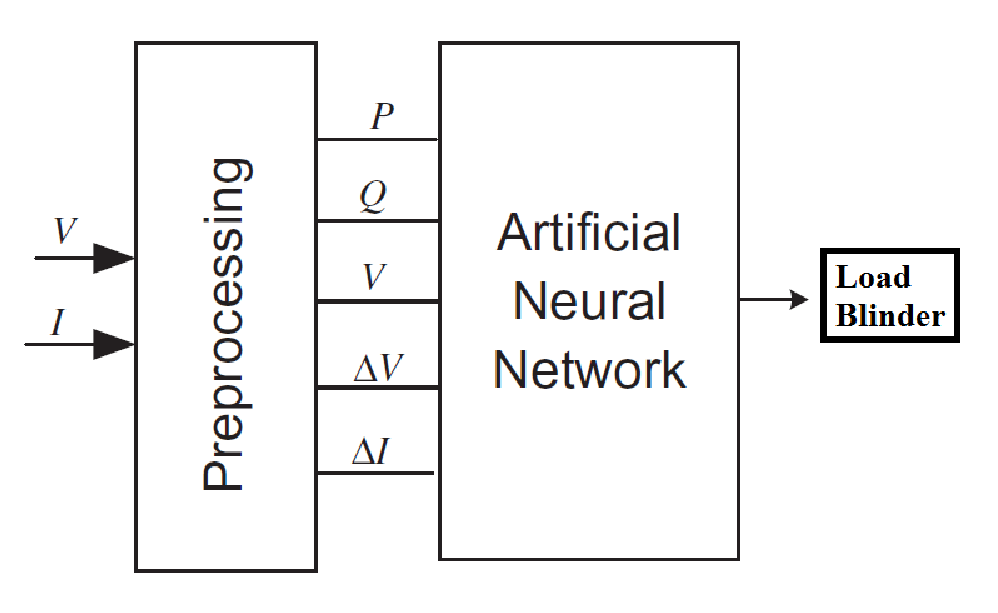
\includegraphics[scale=0.7]{fig7}\caption{Creation of adaptive load blinder in \citep{zadeh2011adaptive} \label{fig:Creation-of-adaptive}}
\par\end{centering}
\end{figure}

In \citep{Nikolaidis2016,Nikolaidis}, the authors propose changing
zone 3 reach during emergency conditions to prevent distance protection
misoperation if certain system conditions are met. If those system
conditions are met, zone 3 protection reach will be shrunk to zone
2 which in turn gives maximum security. During stressed system conditions,
the impedance seen by the local relay approaches the original zone
3 border, whether this border is MHO characteristics or polygonal
one. The authors propose to define a fourth protection zone, called
third zone proximity area (TZPA), as well as a fifth protection zone,
called third zone modification area (TZMA), to change zone 3 protection
reach based on certain criteria. The TZMA is a region within TZPA
but closer to zone 3 protection zone. The authors provided rules on
how to set both TZMA and TZPA. Once the impedance enters this TZPA
and crosses zone 3 fast enough, the fault will be declared. However,
if the impedance enters TZPA and stays within TZPA, the TZMA logic
will be put into action. Zone 3 protection will be shrunk to zone
2 if the impedance crosses TZMA within a minute. This one minute is
used to adjust for restorative corrective forces of the gird such
as generator excitation controls and transformer load tap changer.
In summary, zone 3 protection will only be changed if the impedance
crosses TZMA with a certain rate within a specified time delay once
it starts changing in TZPA. These ideas are illustrated in Figure
\ref{fig:TZMA-and-TZPA}. Although, the approach is very promising,
a fast evolving system instability could mislead the scheme. Additionally,
it can be seen that the approach proposed sacrifices dependability
for security as evident by shrinking zone 3; if a fault occurs within
the original zone 3 protection zone beyond the original zone 2 reach
after zone 3 protection zone is shrunk, the approach proposed by the
authors will rely heavily on the closest relay and circuit breaker
to clear the fault. However, if this relay or circuit breaker fails
to clear the fault, the fault will go uncleared worsening the already
stressed system conditions. Lastly, the proposed algorithm will fail
definitely in case the impedance stays within TZPA, suddenly jumps
to original zone 3 due to zone 3 fault before the time delay expires
then stays in zone 3 after fault clearing due to line heavy loading
conditions. 
\begin{figure}[h]
\begin{centering}
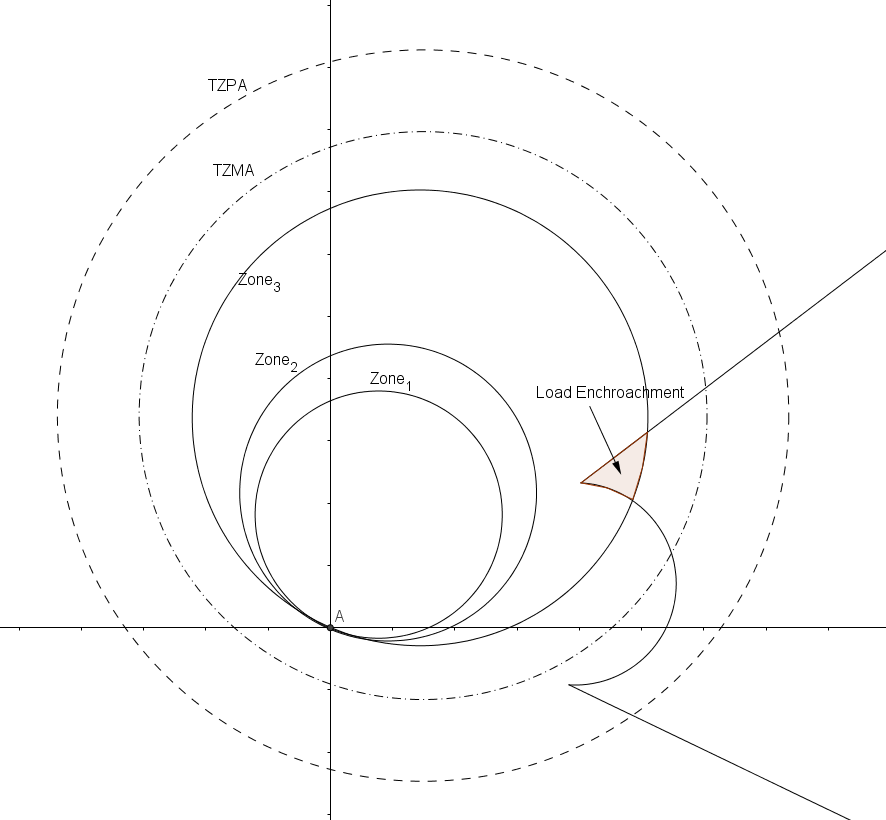
\includegraphics[scale=0.6]{fig8}\caption{TZMA and TZPA of the method in \citep{Nikolaidis2016}\label{fig:TZMA-and-TZPA} }
\par\end{centering}
\end{figure}

Lastly, the authors in \citep{ma2016adaptive} proposed to identify
power flow overload based on a newly proposed concept. This concept
is based on the phasor relationships in the complex phasor plane.
The paper only differentiates between three phase faults and overloads
as overloads are three phase balanced phenomenon. Since the paper
only aims to distinguish three phase faults from overload, any three
phase fault on a transmission line can be analyzed without the need
of information from the other end of line. This is due to the fact
that the arc voltage is not affected by the infeed fault current making
the fault point grounded through the arc resistance. This property
is used to derive the criterion to differentiate between three phase
faults and overloads based on an impedance criterion that can be adaptively
adjusted using the measured phase angle between the voltage and current
at the relay location as well as a constant safety factor. However,
the method is not applicable when a three phase fault occurs within
the distance relay reach during an overload condition. Additionally,
it is assumed that all three phase to ground faults involve arc without
the consideration of the other situations when three phase downed
conductors cause such faults which in turn could cause some of the
assumptions used in deriving the impedance criterion to be invalid. 

\textbf{In summary, the use of rate of change of voltages and currents
can prevent the problem of distance protection misoperation in most
occasions but does not fully prevent it. Other methods use previous
operational experience with distance relays to propose solutions to
the problem of distance protection misoperation. However, system conditions
and scenarios that were not previously encountered could mislead those
proposed solutions. The use of high frequency fault generated transients
seems to be a promising area but it is scarcely researched in literature.}

\section{Conclusion}

The problem of distance protection misoperation has been presented.
Various approaches to solve the problem have been surveyed and organized
into three main categories. The methods in each category have been
explained. Additionally, the advantages and disadvantages of each
method have been pointed out. 

The first category is anticipation of distance protection misoperation
in the planning stage. In this category, distance protection misoperation
could be anticipated day ahead based on the forecasted load and generation
as well as contingency conditions. However, due to the large size
of modern day power systems, such anticipation is computationally
intensive. 

The second category is communication assisted protection schemes.
The main idea in this category is that using information from both
ends of the line or information from various substations in the network,
a blocking command can be issued to the affected distance relay. Nevertheless,
these communication assisted protection schemes have not found wide
industry acceptance due to cybersecurity risks as well as the economic
cost that is required to build such systems. 

The third category is modification of the local distance protection
function using local information. The main idea in this family of
solutions is that using operational system experience as well as the
local data, one can tell with certainty that a distance relay is about
to misoperate. By detecting such conditions, a blocking command can
be issued to guard the relay against misoperation. Nevertheless, the
methods in this last category may fail under system conditions that
were not taken into consideration while developing these methods. 

The most appropriate method to mitigate zone 3 misoperation is dependent
on what is the most important factor for the utility company. For
example, one utility company may prefer a communication-assisted scheme
using remote measurements to eliminate the possibility for distance
protection misoperation while accepting the cybersecurity vulnerabilities
that are introduced. Another utility may not be willing to accept
the cybersecurity risks or the cost of constructing such scheme and
requires a solution using local measurements or minimum remote measurements.
The authors think that methods which use local relay data are worthy
of research attention as cybersecurity threats are becoming a major
concern. 

\bibliographystyle{IEEEtran}
\phantomsection\addcontentsline{toc}{section}{\refname}\bibliography{newlit,references_used_in_proposal}

\end{document}
